\documentclass{beamer}
\usetheme{Boadilla}

\usepackage{amsmath,amssymb}
\usepackage{graphicx}
\usepackage{gvv}
\usepackage{listings}
\usepackage{xcolor}

% Code style
\lstset{
  basicstyle=\ttfamily\scriptsize,
  breaklines=true,
  frame=single,
  numbers=left,
  numberstyle=\tiny,
  keywordstyle=\color{blue},
  commentstyle=\color{green!50!black},
  stringstyle=\color{red!60!black},
  showstringspaces=false
}

\title{Matrix 3.2.31}
\author{ai25btech11015 -- M Sai Rithik}
\date{}

\begin{document}
\frame{\titlepage}

% --- Question ---
\begin{frame}
\frametitle{Question (3.2.31)}
A triangle \(ABC\) can be constructed in which
\[
\angle B = 60^\circ,\qquad \angle C = 45^\circ,
\]
and
\[
AB + BC + AC = 12\ \text{cm}.
\]
\end{frame}

% --- Setup ---
\begin{frame}
\frametitle{Setup}
Let the sides be
\[
a = BC,\quad b = CA,\quad c = AB,
\]
with opposite angles \(A,B,C\).

The equations are:
\begin{align}
a + b + c &= 12, \\
-\,a + (\cos C)b + (\cos B)c &= 0, \\
(\sin C)b - (\sin B)c &= 0.
\end{align}
\end{frame}

% --- Augmented Matrix ---
\begin{frame}
\frametitle{Augmented Matrix}
Substituting \(\cos60=\tfrac12,\;\sin60=\tfrac{\sqrt3}{2},\;\cos45=\sin45=\tfrac{\sqrt2}{2}\):
\[
\left[
\begin{array}{ccc|c}
1 & 1 & 1 & 12 \\[4pt]
-1 & \tfrac{\sqrt{2}}{2} & \tfrac{1}{2} & 0 \\[6pt]
0 & \tfrac{\sqrt{2}}{2} & -\tfrac{\sqrt{3}}{2} & 0
\end{array}
\right].
\]
\end{frame}

% --- RREF Steps ---
\begin{frame}
\frametitle{RREF Step}
Add row 2 to row 1:
\[
R_1 \gets R_1 + R_2
\]
\[
\left[
\begin{array}{ccc|c}
0 & 1+\tfrac{\sqrt{2}}{2} & 1+\tfrac{1}{2} & 12 \\[6pt]
-1 & \tfrac{\sqrt{2}}{2} & \tfrac{1}{2} & 0 \\[6pt]
0 & \tfrac{\sqrt{2}}{2} & -\tfrac{\sqrt{3}}{2} & 0
\end{array}
\right].
\]
\end{frame}

% --- Relations ---
\begin{frame}
\frametitle{Relations}
From RREF we get:
\[
a = c\cdot\frac{\sqrt{3}+1}{2}, \qquad
b = c\cdot\frac{\sqrt{6}}{2}.
\]

Using \(a+b+c=12\):
\[
c\left(\frac{\sqrt{3}+1}{2}+\frac{\sqrt{6}}{2}+1\right) = 12,
\]
so
\[
c = \frac{24}{\sqrt{3}+\sqrt{6}+3}.
\]
\end{frame}

% --- Final Values ---
\begin{frame}
\frametitle{Final Values}
Substituting:
\[
b = \frac{12\sqrt{6}}{\sqrt{3}+\sqrt{6}+3},\qquad
a = \frac{12(\sqrt{3}+1)}{\sqrt{3}+\sqrt{6}+3}.
\]

Numerically:
\[
a \approx 4.565,\quad b \approx 4.093,\quad c \approx 3.342.
\]
Check: \(a+b+c = 12\).
\end{frame}

% --- Plot Instructions ---
\begin{frame}
\frametitle{Plot}
Place
\[
B=(0,0),\quad C=(a,0).
\]
Then
\[
A = (c\cos B,\; c\sin B).
\]
\end{frame}

\begin{figure}[h!]
    \centering
    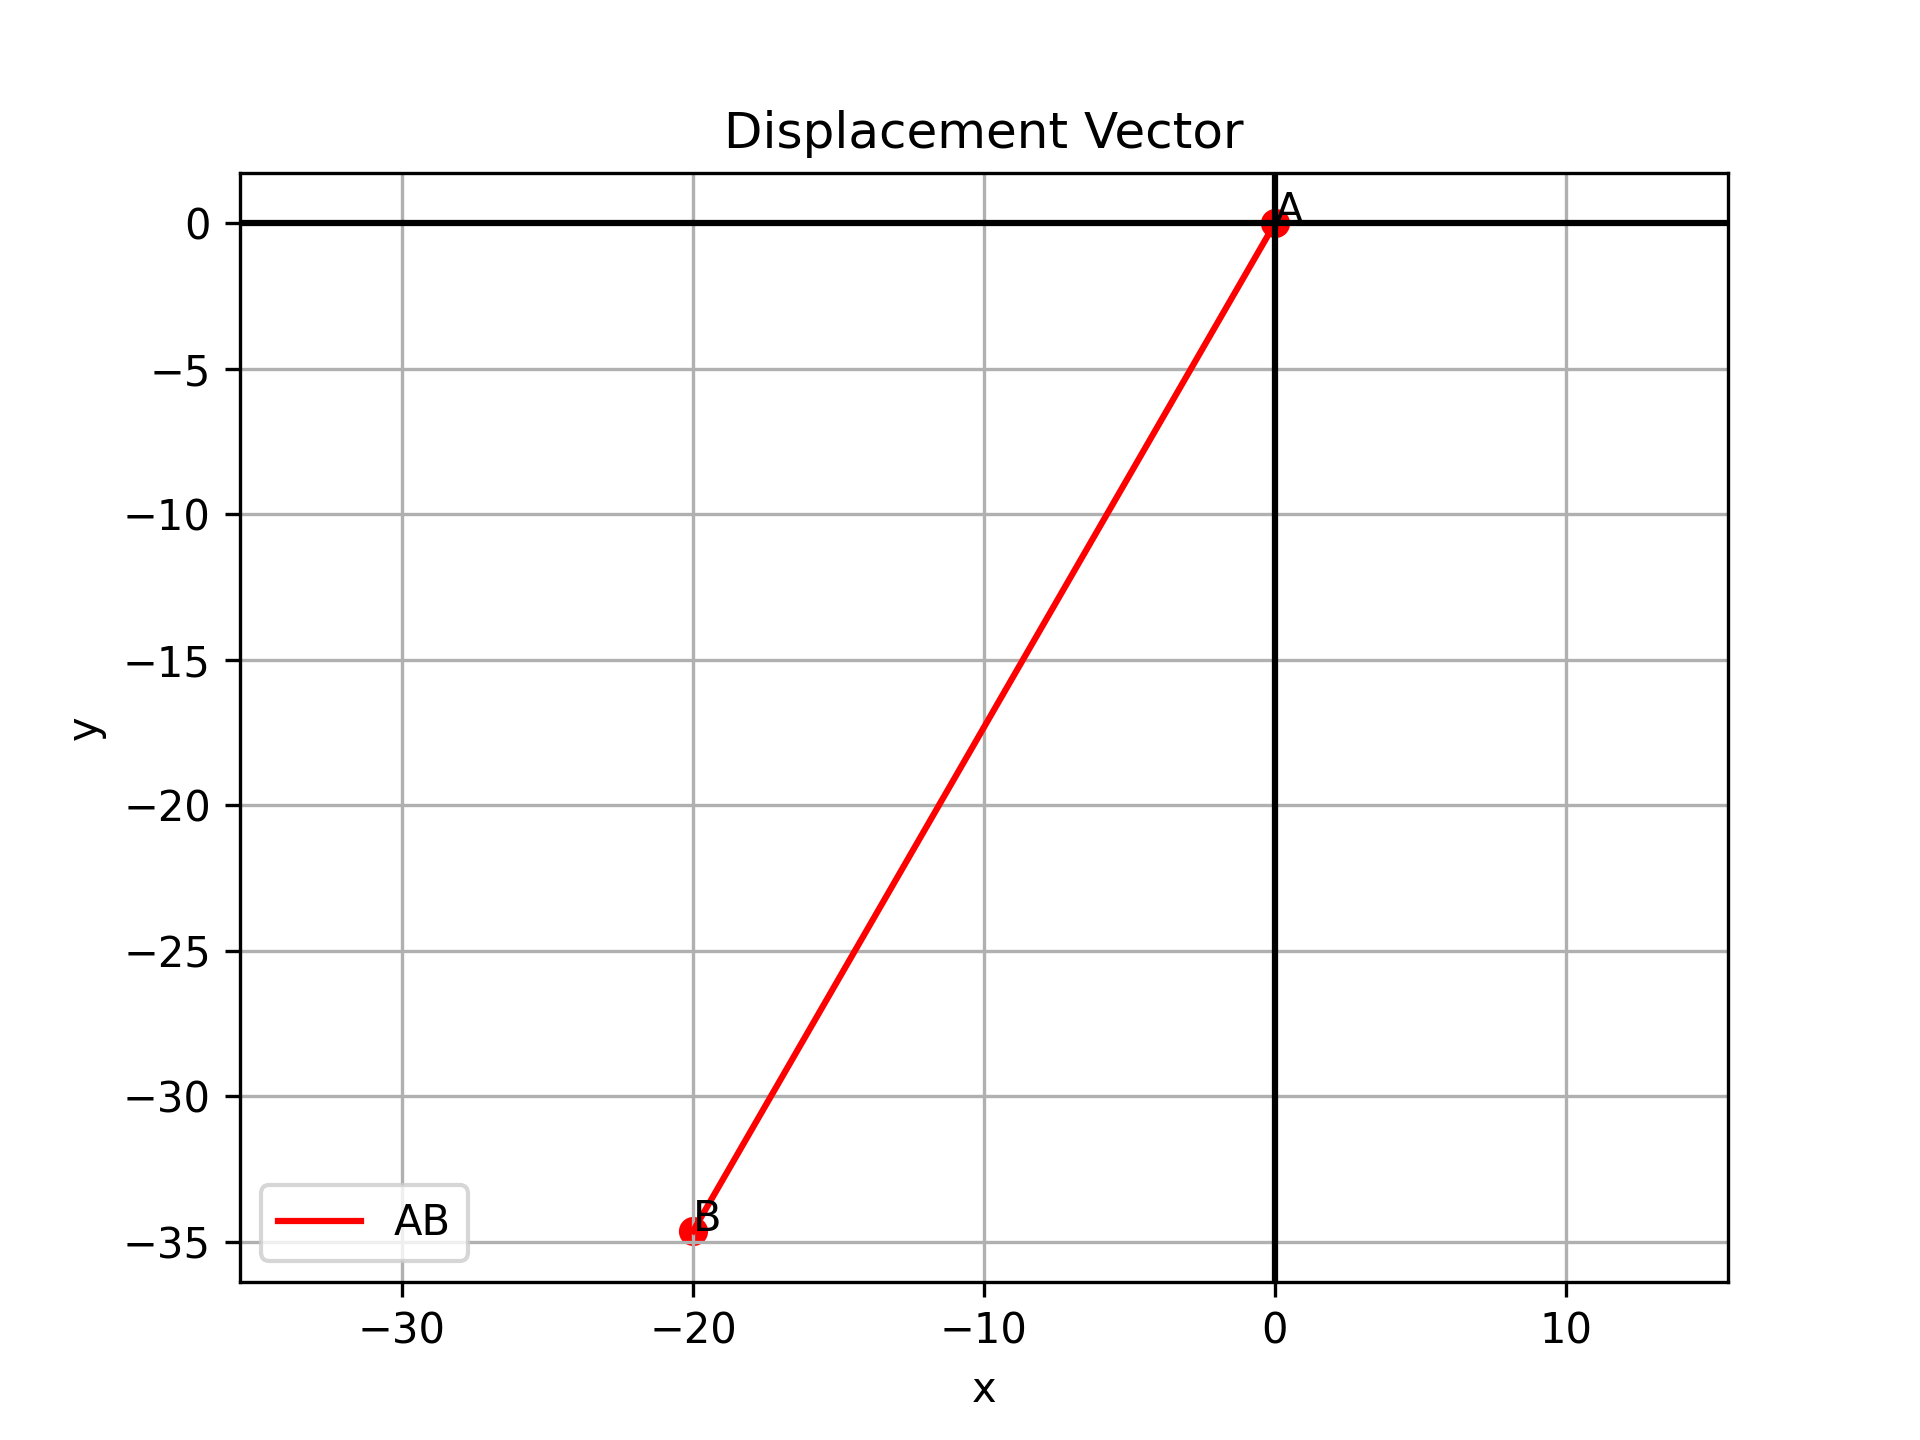
\includegraphics[width=0.65\linewidth]{figs/fig.png}
    \caption{Triangle formed by points $A$, $B$, and $C$.}
\end{figure}

\end{document}
